\ifdefined\iscombined
	\lecturetitle{MC/DC, Structural Testing, and The V Model}
\else
\documentclass{article}
\usepackage{changepage}
\usepackage{centernot}
\usepackage{listings}
\usepackage{amsthm}
\usepackage{braket}
\usepackage{comment}
\usepackage{algorithm}
\usepackage{algpseudocode}
\usepackage{amsmath}
\usepackage{amsfonts}
\usepackage{sectsty}
\usepackage{hyperref}
\usepackage{fancyhdr}
\usepackage[top=1in,bottom=1in,left=1in,right=1in]{geometry}
\usepackage{float}
\usepackage{graphicx}
\usepackage{tabularx}
\usepackage{mathtools}
\usepackage{tikz}
\usetikzlibrary{positioning}

\date{
	\vspace{-.75em}
	{\large \today}
}

\title{
	\vspace*{-1.5em}
	{\Huge Lecture 13} \\
	\vspace{-1em}
	\rule{\textwidth/4}{.01em} \\
	\vspace{-.25em}
	{\Large MC/DC, Structural Testing, and The V Model}
	\vspace{-.75em}
}

\author{
	{\large Matthew Farah}
}

\hypersetup{
	colorlinks=true,
	linkcolor=blue,
	filecolor=magenta,
	urlcolor=blue,
	citecolor=blue,
	anchorcolor=blue
}

\fancyhead{}
\fancyhead[L]{\today}
\fancyhead[R]{Lecture 13 - MC/DC, Structural Testing, and The V Model}

\setlength{\parindent}{0cm}

\lstset{
	basicstyle=\ttfamily\small,
	frame=single,
	tabsize=4,
	breaklines=true,
	numbers=left,
	numberstyle=\tiny,
	numbersep=8pt,
	xleftmargin=1.5em,
	framexleftmargin=1.5em
}

\newcounter{example}
\renewcommand{\theexample}{\arabic{example}}

\newenvironment{example}[1][]{
	\refstepcounter{example}
	\begin{adjustwidth}{1.5em}{}
	\noindent\textbf{\ifx&#1&Example \theexample:\else Example \theexample \ (#1):\fi}
	\ignorespaces
}{
	\vspace{.5em}
	\end{adjustwidth}
}

\newcounter{subexample}
\renewcommand{\thesubexample}{\alph{subexample}}

\newenvironment{subexample}{
	\setcounter{step}{0}
	\refstepcounter{subexample}
	\vspace{1em}\par\noindent
	\begin{adjustwidth}{1.5em}{}
	\noindent\textbf{(\thesubexample)}
	\ignorespaces
}{
	\par
	\vspace{1em}
	\end{adjustwidth}
}

\newenvironment{solution}{
	\vspace{.5em}
	\par
	\begin{adjustwidth}{1.5em}{}
	\textbf{{Solution:}}
	\par
	\vspace{.5em}
}{
	\vspace{1em}
	\end{adjustwidth}
}

\newcounter{step}
\renewcommand{\thestep}{\Roman{step}}

\newenvironment{step}{
	\refstepcounter{step}
	\vspace{1em}\par\noindent
	\ignorespaces\noindent\textbf{(\thestep)}
	\ignorespaces
}{
	\par
	\vspace{1em}
}

\sectionfont{\fontsize{12}{12}\bfseries}
\subsectionfont{\fontsize{10}{12}\normalfont}
\subsubsectionfont{\fontsize{10}{12}\normalfont}

\begin{document}

\maketitle
\pagestyle{fancy}

\fi

\begin{itemize}
	\item MC/DC typically requires $n + 1$ tests for a program with $n$ inputs.
	\begin{itemize}
		\item If not, it needs more than that.
	\end{itemize}
	\item MC/DC works differently when testing objects and source code.
	\begin{itemize}
		\item Source code coverage $\centernot\implies$ object code coverage.
		\begin{itemize}
			\item \emph{Note: the prof never really defined what object code is AFAIK, but it probably just means something the program/system compiles to}.
		\end{itemize}
	\end{itemize}
	\item Structural coverage may refer to any of:
	\begin{itemize}
		\item Statement coverage.
		\item Branch coverage.
		\item Condition coverage.
		\item MC/DC coverage.
		\item Path coverage.
	\end{itemize}
	\item The criterion of a structural test refers to what coverage it is.
	\item Structural tests should be designed to consider:
	\begin{itemize}
		\item What happens if a loop is never executed.
		\item A loop is only executed once.
		\item A loop is executed some arbitrary number of times.
	\end{itemize}
	\item Structural tests should also be designed to force:
	\begin{itemize}
		\item An immediate success.
		\item An eventual success.
		\item An immediate failure.
	\end{itemize}
	\item A criterion `subsumes' another one if satisfying it implies satisfying the other.
	\begin{itemize}
		\item I.E. $A$ subsumes $B$ if satisfying $A$ implies satisfying $B$.
	\end{itemize}
	\item If a criterion subsumes another, it is considered better.
	\begin{itemize}
		\item Doesn't mean it will necessarily encounter the same failures.
	\end{itemize}
	\item Subsumption is transitive.
	\begin{itemize}
		\item I.E. If $A$ subsumes $B$ and $B$ subsumes $C$ then $A$ subsumes $C$.
	\end{itemize}
	\item Structural tests criteria are ordered in terms of subsumption as follows:
	\begin{itemize}
		\item Path coverage subsumes MC/DC coverage.
		\item MC/DC coverage subsumes both branch and condition coverage.
		\item Branch coverage subsumes statement coverage.
	\end{itemize}
\end{itemize}

\begin{center}
	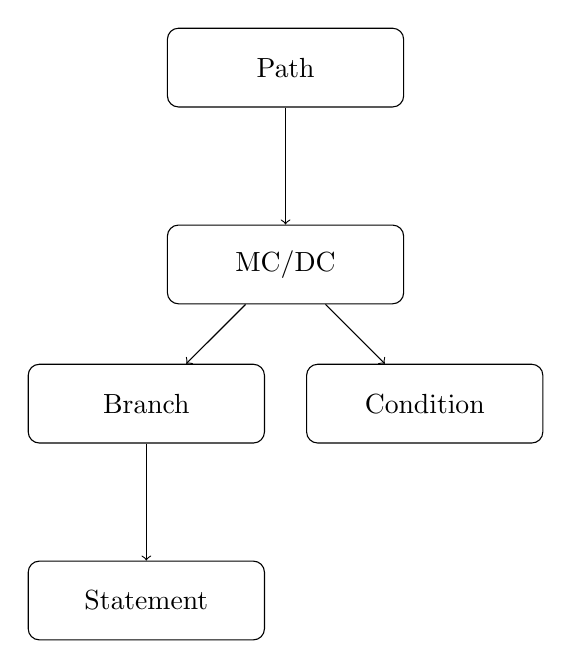
\begin{tikzpicture}
		[
			node distance=2.5cm,
			every node/.style={draw, rectangle, rounded corners, minimum width=3cm, minimum height=1cm, align=center},
			every edge/.style={draw, ->, >=latex', thick}
		]

		\node (path) {Path};
		\node (mcdc) [below of=path] {MC/DC};
		\node (branch) [below left of=mcdc] {Branch};
		\node (condition) [below right of=mcdc] {Condition};
		\node (statement) [below of=branch] {Statement};
	
		\draw[->] (path) -- (mcdc);
		\draw[->] (mcdc) -- (branch);
		\draw[->] (mcdc) -- (condition);
		\draw[->] (branch) -- (statement);
	\end{tikzpicture}
\end{center}

\begin{itemize}
	\item Complexity metrics measure how difficult code is to test.
	\begin{itemize}
		\item For example, control-flow complexity or state behaviour complexity.
	\end{itemize}
	\item The Software Development Life-Cycle (SDLC) refers to a range of different possible development approaches teams can/should follow to work optimally.
	\begin{itemize}
		\item An SDLC models refer to some such specified approach.
	\end{itemize}
	\item The V-model is an SDLC model focused primarily on developing the system's requirements.
	\item The V-model divides up development into two main phases, done in the following order:
	\begin{enumerate}
		\item Verification.
		\begin{itemize}
			\item Involves insuring the system is built to do the right job.
			\begin{itemize}
				\item Done by speaking with clients.
			\end{itemize}
		\end{itemize}
		\item Validation.
		\begin{itemize}
			\item Involves insuring the system does its job right.
			\begin{itemize}
				\item Done by checking if system meets some set of standards. \\
			\end{itemize}
		\end{itemize}
	\end{enumerate}

	\item \emph{Aside: The difference between verification and validation is pretty easy to miss but you're supposed to think about it like, if you're trying to help someone travel, verification is about making sure that a car is good for them and validation is making sure the engine starts.}
	\begin{itemize}
		\item \emph{Second aside: I hate learning about project management but I cannot escape it someone save me.}
	\end{itemize}
\end{itemize}

\ifdefined\iscombined
	\newpage
\else
	\end{document}
\fi
